% Fichier LaTeX enrichi avec images UPDF
% Exercice 5 - Amérique du Nord ^
% 19 points

\documentclass[12pt]{article}
\usepackage[utf8]{inputenc}
\usepackage[T1]{fontenc}
\usepackage[french]{babel}
\usepackage{graphicx}
\usepackage{amsmath}
\usepackage{amssymb}
\usepackage{geometry}
\geometry{a4paper, margin=2cm}

\begin{document}

\section*{Exercice 5 (19 points)}

% Images de l'exercice
\begin{center}
\includegraphics[width=0.8\textwidth]{images/dnb_2025_06_ameriquenord_5_Image_011.gif}
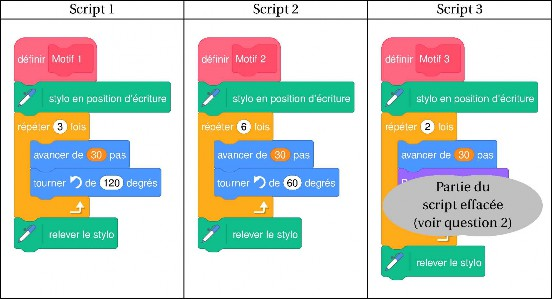
\includegraphics[width=0.8\textwidth]{images/dnb_2025_06_ameriquenord_5_Image_012.jpg}
\includegraphics[width=0.8\textwidth]{images/dnb_2025_06_ameriquenord_5_Image_013.gif}
\end{center}

\begin{enumerate}
\item Les scripts 1 et 2 permettent chacun d'obtenir un des dessins ci-dessous. Associer chacun des scripts à son dessin.

\begin{center}
\begin{tabularx}{\linewidth}{|*{2}{>{\centering \arraybackslash}X|}}\hline
Dessin 1&Dessin 2\\ \hline
\psset{unit=0.9cm}
\begin{pspicture}(-1.5,-1.5)(1.5,1.3)
\pspolygon(1.5;0)(1.5;60)(1.5;120)(1.5;180)(1.5;240)(1.5;300)
\end{pspicture}&
\psset{unit=1cm}
\begin{pspicture}(-1.8,-1)(1.8,1.8)
\pspolygon(1.4;-30)(1.4;90)(1.4;210)
\end{pspicture}\\ \hline
\end{tabularx}
\end{center}


\begin{minipage}{0.55\linewidth}

\item Le script 3 permet d'obtenir le losange ci-contre.

La partie du script effacée contient les 3 instructions A, B et C ci-dessous.

Sur votre copie, recopier dans le bon ordre les instructions cachées.

\item Calculer la fréquence de l'affichage \og Voici le dessin! \fg{}.

\item Pourquoi ce résultat est-il différent de celui obtenu à la question 5 ?

\end{enumerate}

\end{document}
